\documentclass[11pt]{article}
\usepackage[a4paper, total={6in, 8.5in}]{geometry}
\usepackage[english]{babel}
\usepackage{graphicx}
\usepackage{hyperref}
\usepackage[onehalfspacing]{setspace}
\usepackage{float}
\usepackage{titlepic}
\usepackage{listings}
% \usepackage{xcolor}
\usepackage{amsmath}
\usepackage{amsfonts}
\usepackage{scrlayer-scrpage}
\usepackage{csquotes}
\usepackage{blkarray}
\usepackage{mwe}
\usepackage{algorithm}
\usepackage{algorithmic}
\usepackage{esvect}
\usepackage{physics}
\usepackage[table,xcdraw]{xcolor}


\usepackage[style=authoryear, backend=biber]{biblatex}
\usepackage{amssymb}
\addbibresource{references.bib}
\cfoot*{\pagemark}

\DeclareMathOperator*{\argmax}{arg\,max}
\DeclareMathOperator*{\argmin}{arg\,min}
\newcommand{\E}{\mathrm{E}}
\newcommand{\Var}{\mathrm{Var}}
\newcommand{\Cov}{\mathrm{Cov}}



\begin{document}
    \title{Autonomous Systems - Perception, Markov Localisation}
    \date{04/2021}
    \author{Rupp Matthias}
    \maketitle
    \thispagestyle{empty}
    \vspace{2 cm}
    \begin{figure}[H]
        \centering
        
\includegraphics[width = 6cm]{Logo-A3}\label{fig:logo}
    \end{figure}
    \pagebreak

    \ohead{Rupp Matthias}
    \tableofcontents
    \thispagestyle{empty}
    \clearpage

    \definecolor{codegreen}{rgb}{0,0.6,0}
    \definecolor{codegray}{rgb}{0.5,0.5,0.5}
    \definecolor{codepurple}{rgb}{0.58,0,0.82}
    \definecolor{backcolour}{rgb}{0.95,0.95,0.92}

    \lstdefinestyle{mystyle}{
        backgroundcolor=\color{backcolour},
        commentstyle=\color{codegreen},
        keywordstyle=\color{magenta},
        numberstyle=\tiny\color{codegray},
        stringstyle=\color{codepurple},
        basicstyle=\ttfamily\footnotesize,
        breakatwhitespace=false,
        breaklines=true,
        captionpos=b,
        keepspaces=true,
        numbers=left,
        numbersep=5pt,
        showspaces=false,
        showstringspaces=false,
        showtabs=false,
        tabsize=2
    }
    \lstset{style=mystyle}

    NOTE: Octave was used to solve this exercise.
    Since Octave-indices start with $1$, not $0$, all indices were incremented by one.
    So, the cells go from $1$ to $50$, and the cells where pillars are located where also shifted by one.
    This does not change the end result, but should be kept in mind when reading this documentation.

    \section{Description of models used}\label{sec:models}
    Two models need to be determined to properly calculate the robot's movements: the movement model and the measurement model.

    \subsection{Movement model}\label{subsec:movem}
    The movement model for this exercise is rather easy.
    The robot moves a certain distance with a certain probability, with the distances being $3, 4, 5, 6, 7$ and the probability being $0.1, 0.2, 0.4, 0.2, 0.1$, respectively.
    These values are saved in a vector with two rows, the first row containing the distance values and the second row containing the probabilities for said distances.
    This way, by taking a column of the vector, both the distance and the probability for the robot moving said distance can be extracted.
    This can be used, together with the "old" posteriors of the preceding steps, to calculate the priors.

    \subsection{Measurement model}\label{subsec:measurem}
    The measurement model is more complex.
    First off, there is a measurement error, with a uncertainty of $\pm 1$ cell.
    The actual distance is measured with a probability of $0.5$, with one cell more or less being measured with a probability of $0.25$.
    Secondly, the robot can only measure the next pillar it can see.
    Pillars are placed on cells $5, 14, 21, 32, 46$, so if a robot stands on cell $3$, it can see the pillar on cell $5$, but not the one on cell $14$.
    This, in turn, means that a distance measurement of, say, $11$ cannot have happened on cell $3$, even though there is a pillar on cell $14$, since cell $5$ blocks the measurement.
    The robot will also not measure any pillars that are on the same cell as him, which also means that there will be no distance with value $0$ measured.\newline
    All this leads to a measurement model that is built as follows.
    \begin{enumerate}
        \item Create a $N x N$ matrix, where $N$ is the number of cells ($50$ in this exercise).
        Note that the matrix could be chosen smaller in this exercise, but a $N x N$ matrix could capture measurements from each cell to every other cell, so it will be used.
        \item Let the index of the matrix row be $r$ and the index of the matrix column be $c$
        \item For each matrix cell $r,c$, enter the probability that the robot measured the distance $c$ from the cell $r$ with $0.5$
        \item For the cells $r,c-1$ and $r,c+1$, enter the probability $0.25$, which is the probability of the measurement error (meaning the robot measured on cell less/more than the cell the actual obstacle is in)
    \end{enumerate}
    The result of this process is a $N x N$ matrix from which, using the cell index as $r$ and the measured distance as $c$, the probability that this distance was measured from said cell can be extracted from cell $r,c$ of the matrix.
    This matrix, together with a vector containing the measured distances for each step, $5,10,7,2,10$, will be used in the posterior calculation.

    \section{Documentation of procedure}\label{sec:proc}

    For this exercise, we start with a uniform distribution for the robot's placement.
    Since we have $50$ cells, this means a probability of $\frac{1}{50}$ for every cell.
    The robot now takes the first step.
    This means the calculation of the new position based on the movement model.\newline
    \autoref{eq:preq} shows the formula for this process, taken from page 19 of \textcite{merz_autonome_2}.
    \begin{equation}\label{eq:preq}
    \overline{\operatorname{bel}}\left(x_{t}\right)=\sum_{x_{t-1}} p\left(x_{t} \mid u_{t}, x_{t-1}\right) \operatorname{bel}\left(x_{t-1}\right)
    \end{equation}
    We want to calculate the probability (or belief), that we are at the position $x_{t}$ after moving.
    To this end, we take the probability that we have moved to position $x_{t}$ given the movement information $u_{t},x_{t-1}$ and multiply this with the probability that the robot was located at $x_{t-1}$ in the first place.
    We then sum up these calculations for each cell and all movement information to get the probabilities that the robot moved to each cell.\newline
    In this concrete example, where the robot moves $3, 4, 5, 6, 7$ steps with the probabilities $0.1, 0.2, 0.4, 0.2, 0.1$, we go through each cell, calculate into which cells it can move from the cell we are currently looking at, multiply the movement possibilities with the possibility that the robot is located in the current cell in the first place, and remember said possibilities for the cells the robot may have moved to.
    To give a concrete example: the robot is in cell $5$ with a probability of $0.2$.
    It moves $3$ cells with a probability of $0.1$, so the probability that the robot moved to cell $5 + 3 = 8$ from cell $5$ is $0.1 * 0.2 = 0.02$.
    For moving $4$ cells, the calculation is $0.2 * 0.2 = 0.04$ for moving to cell $5 + 4 = 9$ and so on.
    By doing this for every cell and summing up the resulting probabilities (so we sum up all the probabilities that the robot could have moved to a certain cell from any other cell, and we do this for each cell), we get a new distribution of probabilities that shows where the robot might be after having moved.
    These are our priors.
    The next step is for the robot to measure distances.\newline
    How to calculate the robot's position after sensor measurements, also called the posteriors, can be seen in \autoref{eq:posteq}, also from page 19 of \textcite{merz_autonome_2}.
    \begin{equation}\label{eq:posteq}
    \operatorname{bel}\left(x_{t}\right)=\eta p\left(z_{t} \mid x_{t}, M\right) \overline{b e l}\left(x_{t}\right)
    \end{equation}
    What we want to know is the probability that the robot is on certain cell given the measured distance.
    However, we do not know this.
    Instead, we calculate our posteriors by calculating the probability that the robot measured a certain distance $z_{t}$ given his current position $x_{t}$ and the map with our obstacles $M$, which we multiply with the probability that the robot is located at said current position in the first place (which is the prior we calculated in the step before, $\overline{b e l}\left(x_{t}\right)$).
    A concrete example would be: we are at cell $12$ with a probability (the prior) of $0.35$.
    The measured distances, as specified in the task sheet, are $5, 10 , 7 , 2, 10$.
    Assuming we are currently measuring after step $4$, this means we measure a distance of $2$.
    Since the next (and only) pillar the robot can see from cell $12$ is the pillar at cell $14$, the probability that we measured the distance $2$ given the position $12$ and the map with the obstacles is $0.5$, due to our sensor having uncertainties.
    So, the calculation is $0.5 * 0.35 = 0.175$ for cell $12$.\newline
    The principle is the same for all other cells.
    Then, we need to multiply this result with a factor $\eta$, to ensure a sum of $1$ over all posteriors.
    Before calculating this $\eta$, it is a good idea to replace all posteriors which are smaller than a certain value $min_{p}$ with said value $min_{p}$, to get rid of any zeros or very small values.
    $\eta$ can then be calculated with the simple formula $\eta = \frac{1}{sum(posteriors)}$.
    Now, we multiply our posteriors with $\eta$, and have finished the calculation of the posteriors for this step.\newline
    In the next step the robot makes, these posteriors will be used to calculate the priors, and the process repeats.

        \section{Results for $5$ steps}\label{sec:results}
        In this section, the prior and posterior plots for $5$ steps will be shown.

        \autoref{fig:prior1} and \autoref{fig:post1} show the priors and posteriors for step $1$.
        \begin{figure}[H]
            \centering
            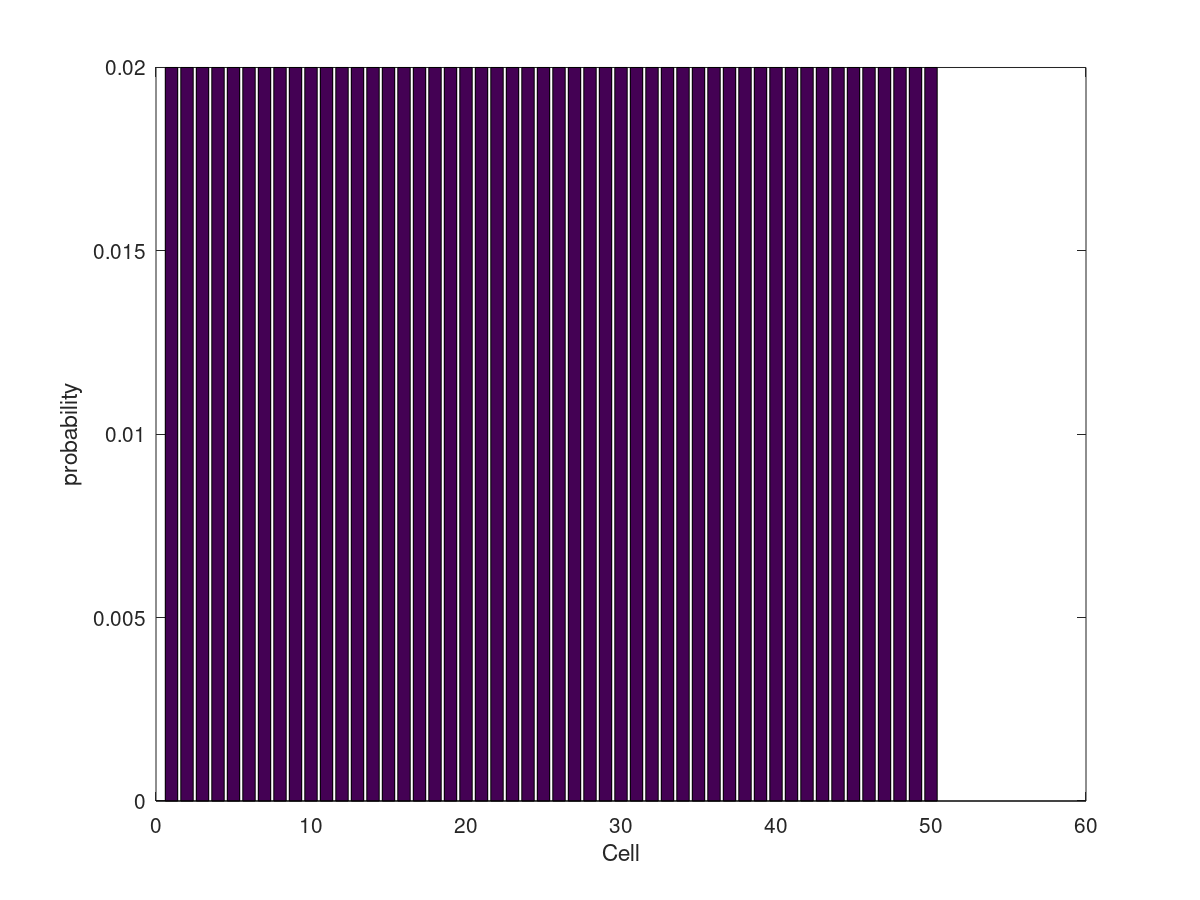
\includegraphics[width=1.0\textwidth]{../images/prior1v2}
            \caption{Prior, step 1}
            \label{fig:prior1}
        \end{figure}
        \begin{figure}[H]
            \centering
            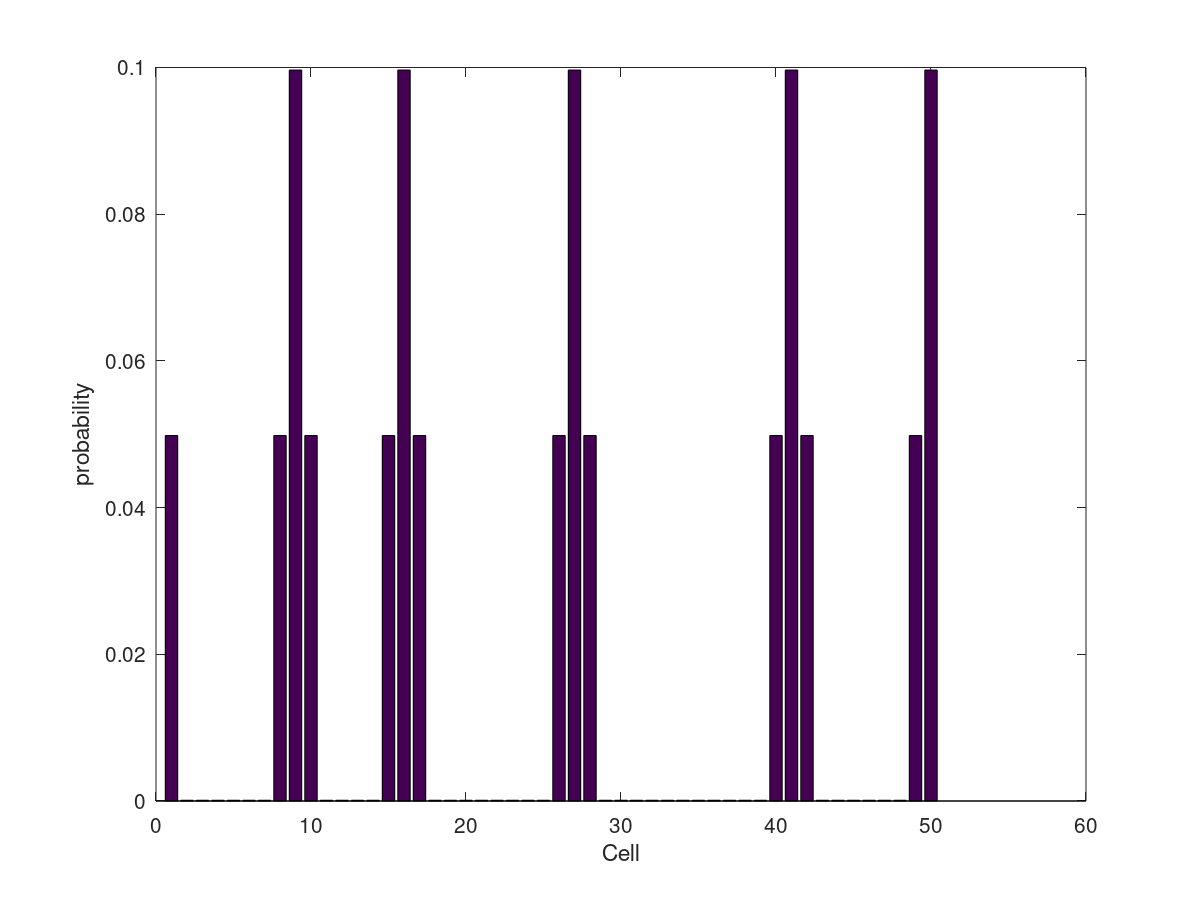
\includegraphics[width=1.0\textwidth]{../images/posterior1v2}
            \caption{Posterior, step 1}
            \label{fig:post1}
        \end{figure}

        \autoref{fig:prior2} and \autoref{fig:post2} show the priors and posteriors for step $2$.
        \begin{figure}[H]
            \centering
            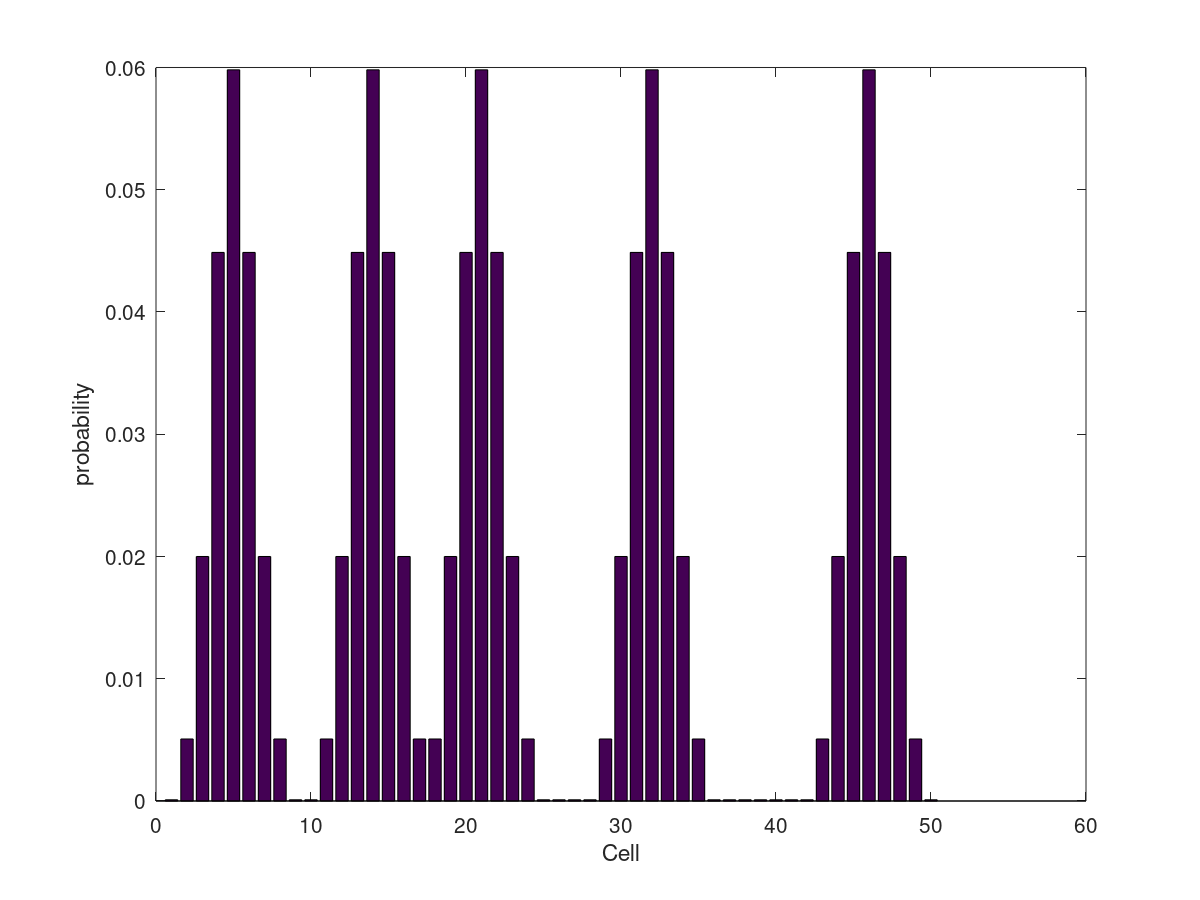
\includegraphics[width=1.0\textwidth]{../images/prior2v2}
            \caption{Prior, step 2}
            \label{fig:prior2}
        \end{figure}
        \begin{figure}[H]
            \centering
            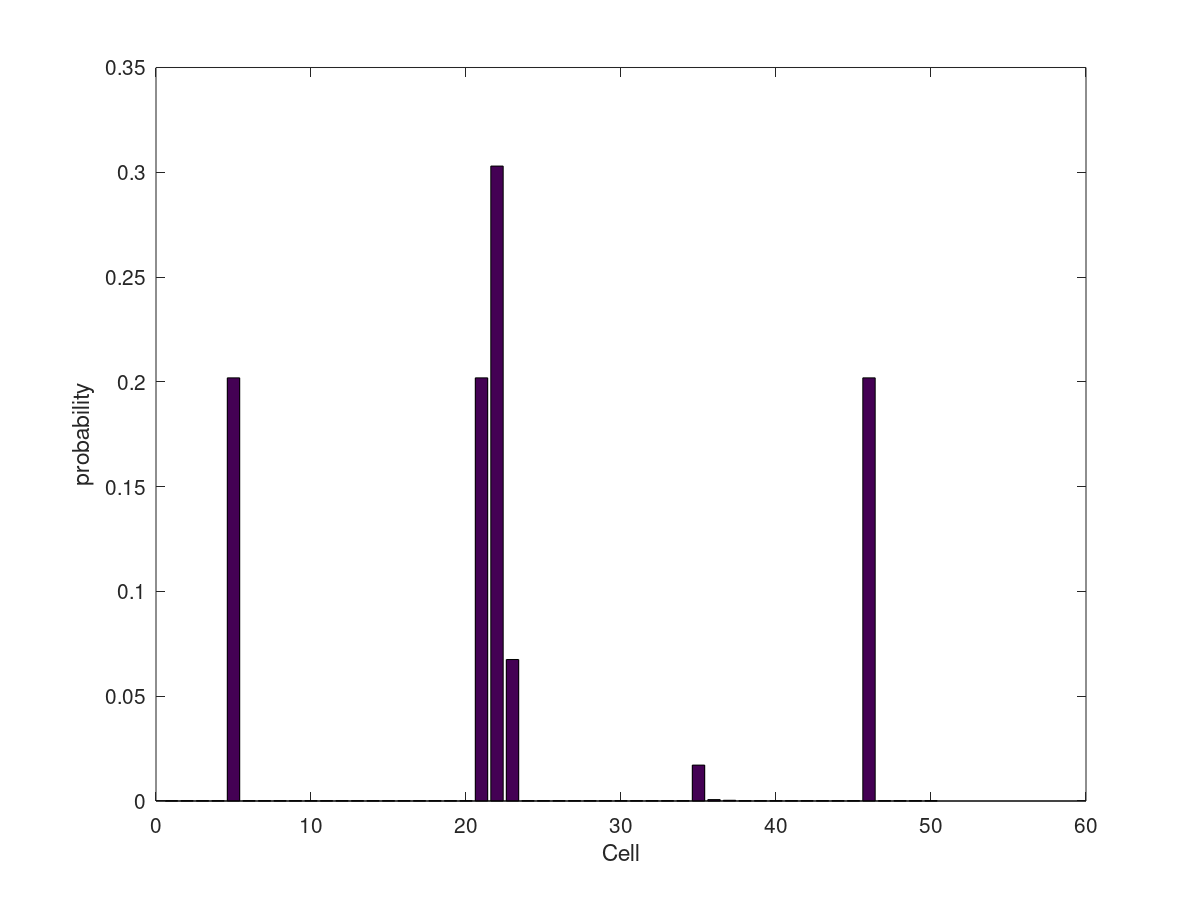
\includegraphics[width=1.0\textwidth]{../images/posterior2v2}
            \caption{Posterior, step 2}
            \label{fig:post2}
        \end{figure}

        \autoref{fig:prior3} and \autoref{fig:post3} show the priors and posteriors for step $3$.
        \begin{figure}[H]
            \centering
            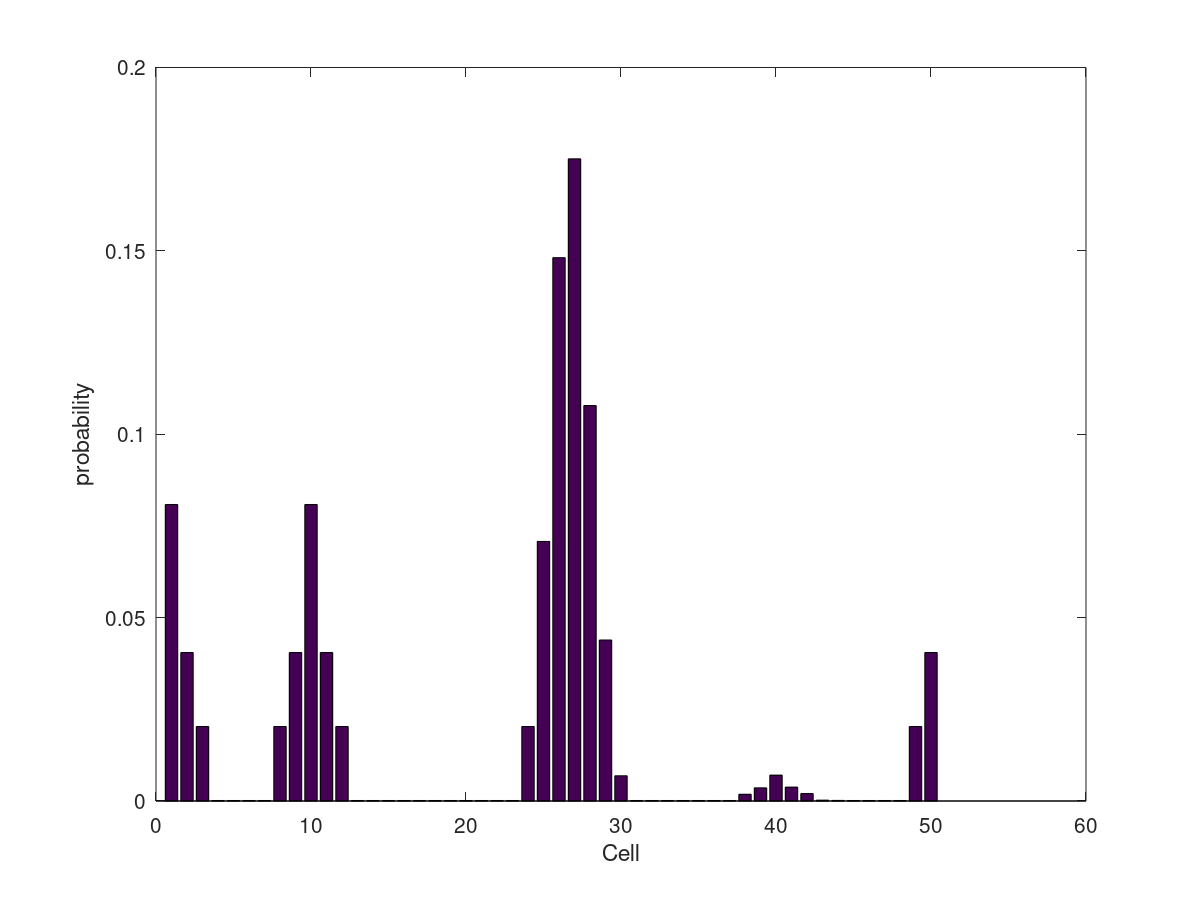
\includegraphics[width=1.0\textwidth]{../images/prior3v2}
            \caption{Prior, step 3}
            \label{fig:prior3}
        \end{figure}
        \begin{figure}[H]
            \centering
            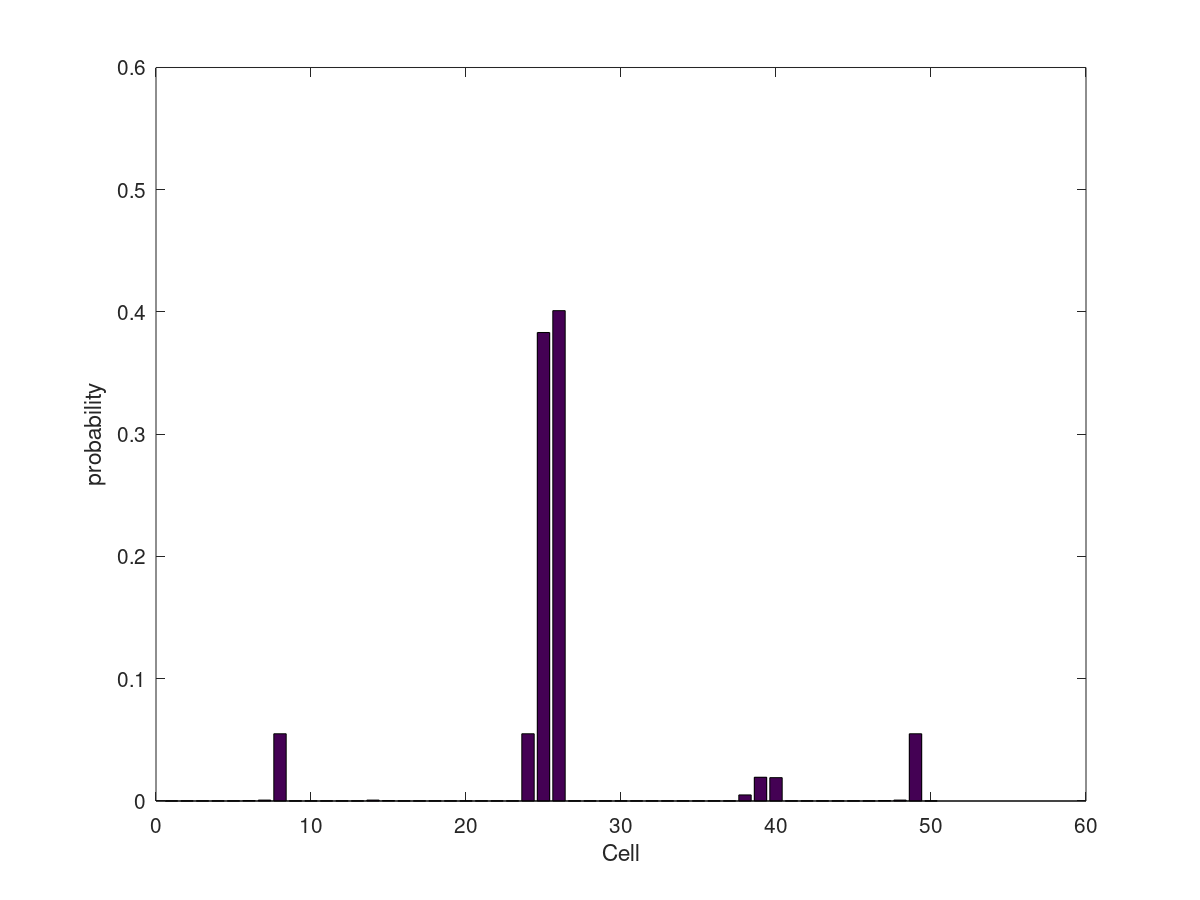
\includegraphics[width=1.0\textwidth]{../images/posterior3v2}
            \caption{Posterior, step 3}
            \label{fig:post3}
        \end{figure}
        \autoref{fig:prior4} and \autoref{fig:post4} show the priors and posteriors for step $4$.
        \begin{figure}[H]
            \centering
            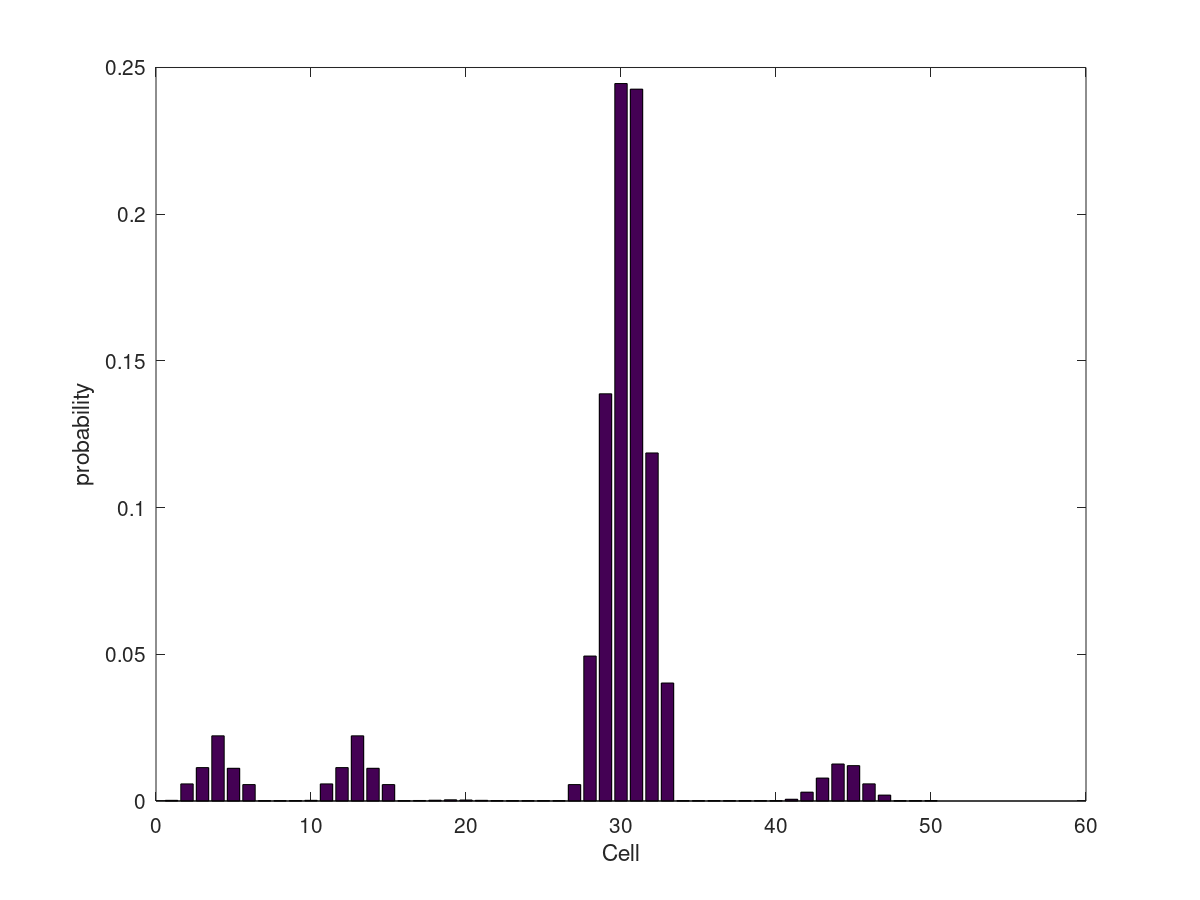
\includegraphics[width=1.0\textwidth]{../images/prior4v2}
            \caption{Prior, step 4}
            \label{fig:prior4}
        \end{figure}
        \begin{figure}[H]
            \centering
            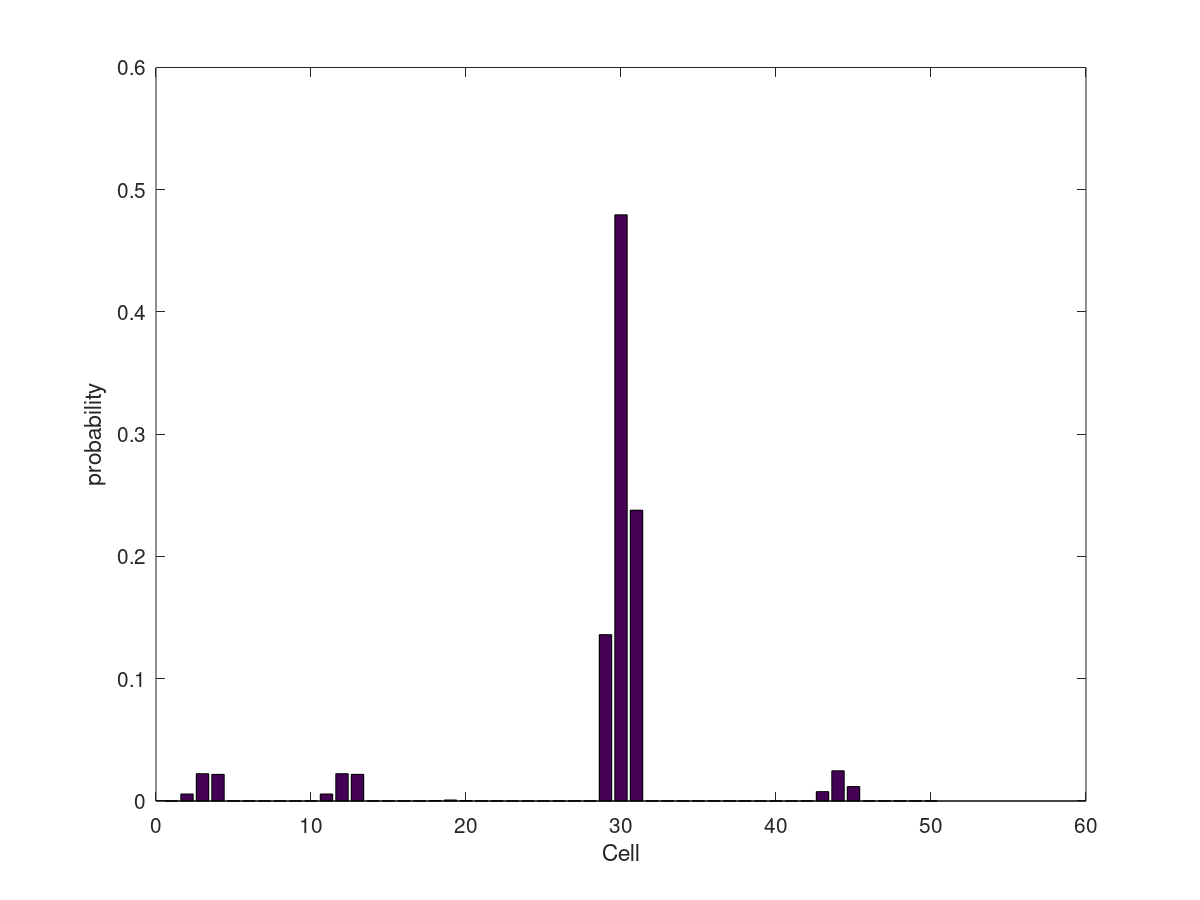
\includegraphics[width=1.0\textwidth]{../images/posterior4v2}
            \caption{Posterior, step 4}
            \label{fig:post4}
        \end{figure}
    Finally, \autoref{fig:prior5} and \autoref{fig:post5} show the priors and posteriors for step $5$.
        \begin{figure}[H]
            \centering
            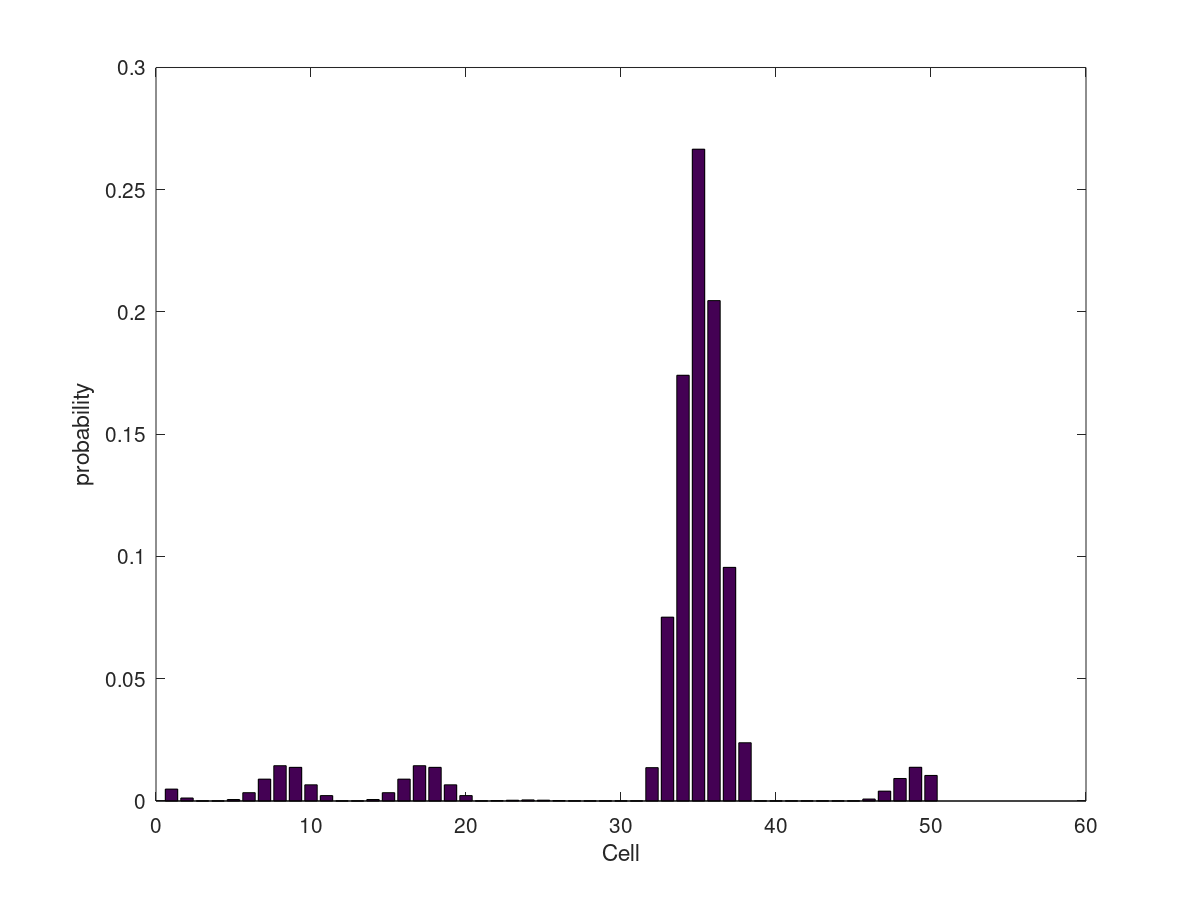
\includegraphics[width=1.0\textwidth]{../images/prior5v2}
            \caption{Prior, step 5}
            \label{fig:prior5}
        \end{figure}
        \begin{figure}[H]
            \centering
            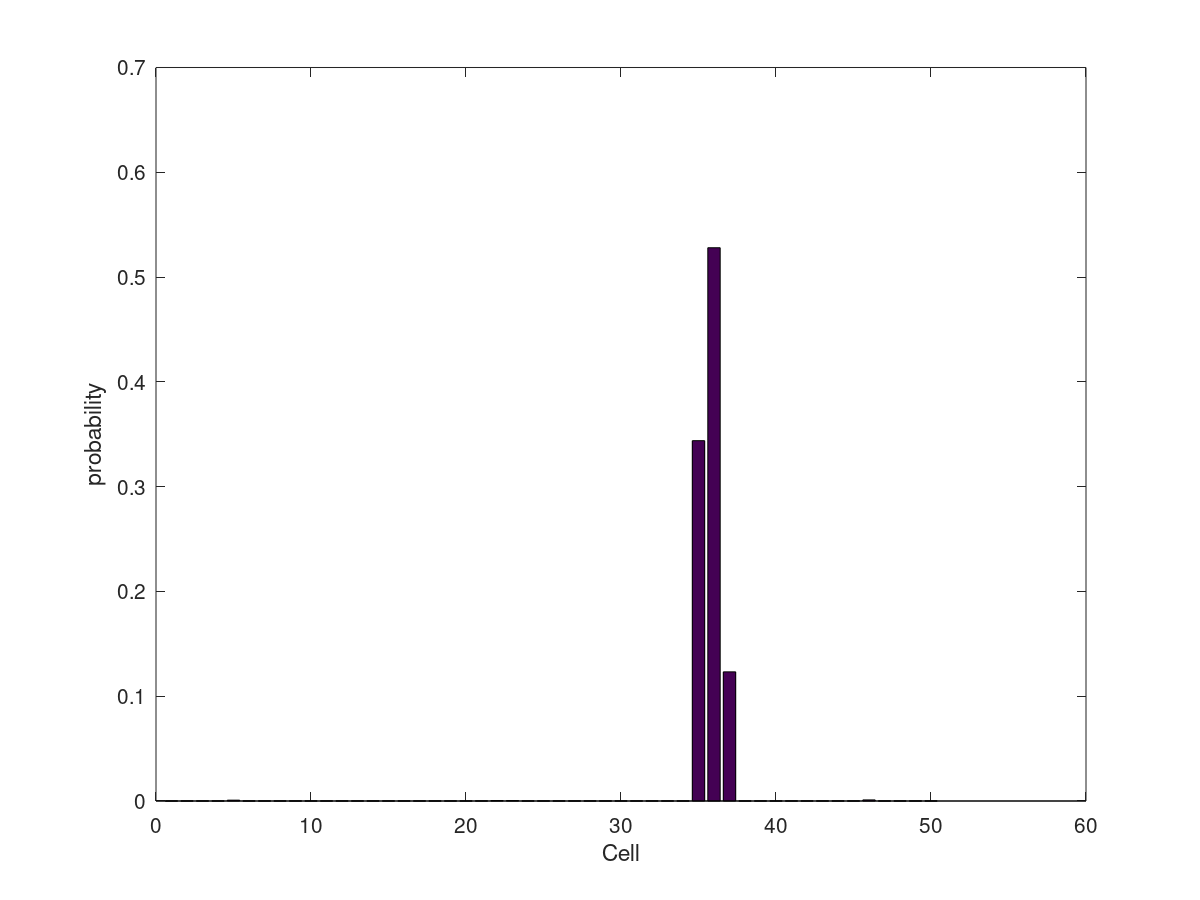
\includegraphics[width=1.0\textwidth]{../images/posterior5v2}
            \caption{Posterior, step 5}
            \label{fig:post5}
        \end{figure}

    \clearpage
    \phantomsection
    \addcontentsline{toc}{section}{References}
    \printbibliography

    \clearpage
    \phantomsection
    \addcontentsline{toc}{section}{List Of Figures}
    \listoffigures


\end{document}